\documentclass[11pt,a4paper]{amsart}

\usepackage{amssymb, amsmath, amsthm, latexsym}
%\usepackage[alphabetic]{amsrefs}
%\usepackage{calrsfs}
%\usepackage{graphicx}
\usepackage{color}
\usepackage{tikz}
\usepackage{bm}
\usepackage{float}



\def\R{{\mathbb R}}
\def\Q{{\mathbb Q}}
\def\Z{{\mathbb Z}}
\def\C{{\mathbb C}}
\def\S{{\mathbb S}}
\def\N{{\mathbb N}}
\def\H{{\mathbb H}}
\def\RP{{\mathbb {RP}}}
\def\p{\partial}
\def\O{\Omega}
\def\pO{{\partial\Omega}}
\def\bO{\overline\Omega}
\def\a{\alpha}
\def\b{\beta}
\def\g{\gamma}
\def\G{\Gamma}
\def\d{\delta}
\def\D{\Delta}
\def\e{\epsilon}
\def\r{\rho}
\def\t{\tau}
\def\l{\lambda}
\def\L{\Lambda}
\def\k{\kappa}
\def\s{\sigma}
\def\th{\theta}
\def\o{\omega}
\def\z{\zeta}
\def\n{\nabla}
\def\T{{\mathcal T}}
\def\X{{\mathcal X}}
\def\area{\mathrm{area}}
\def\dist{\mathrm{\rm dist}}
\def\diag{\mathrm{diag}}
\def\spt{\mathrm{spt\,}}
\def\diam{\mathrm{diam\,}}
\def\dim{\mathrm{dim\,}}
\def\graph{\mathrm{graph\,}}
\def\interior{\mathrm{interior\,}}
\def\diag{\mathrm{diag\,}}
\def\Image{\mathrm{Image}\,}
\def\osc{\mathop{\text{\rm osc}}}

\def\RA{\Rightarrow}
\def\ra{\rightarrow}
\def\rai{\rightarrow\infty}


\newenvironment{solution}{\par\color{blue}\textbf{Solution:}}{\color{black}}

\overfullrule0pt \hoffset=0cm
\parskip=4pt
\parindent=0pt
\baselineskip=20pt

\begin{document}

\thispagestyle{empty}
\begin{center}
\huge
\vspace*{1.0in} MATH2320/3116/6110
\\\vspace{0.5in} \textsc{Assignment 5}
\normalsize
\\\vspace{0.5in} \textsc{By}
\\\vspace{0.1in} \textsc{Zeming Wang}
\\\vspace{0.1in} \textsc{u6114134}
\normalsize
\\\vspace{0.5in} \textsc{Lecture: John Urbas}
\\\vspace{0.1in} \textsc{Tutor: Sophie Chen}
\\\vspace{0.1in} \textsc{Tutorial: Wednesday 5-6 pm}
\normalsize
\\\vspace{0.5in} \textsc{Due: 23 May 2018}
\end{center}

\newpage
\setcounter{page}{1}

% \thispagestyle{empty}

% \begin{center}{\bf MATH2320/3116/6110 Analysis 1 2018}\end{center}



% \medskip

% \begin{center}{\bf Assignment 5}\end{center}

% \medskip

% \begin{center}{\it Due 5pm Monday 21 May 2018}
%  \end{center}

% \smallskip


% {\sl Marking scheme: 45 points + 5 points for presentation. Total 50 points. }

% \medskip



%All questions are of equal value. 

%\bigskip








\bigskip


{\bf 1.} [8+2+8=18 points]  

Let $(X,d)$ be a compact metric space and let $T:X\ra X$ be a distance preserving map,
i.e., 
$$ d(T(x),T(y))=d(x,y) \quad\mbox{for all}\quad x,y\in X. $$
Prove that $T$ is a bijection (i.e., $T$ is one to one and onto).

% Hint: If $T$ is not onto, consider $y\in X\backslash T(X)$. Let $\d=\inf\{d(y,x):x\in T(X)\}>0$.
% Consider the sequence $(y,T(y),T(T(y)),T(T(T(y))),\dots)$ and derive a contradiction.

\begin{proof}
$T$ is obviously an injection, since $T$ is a distance preserving map:
$$ T(x) = T(y) \RA d(T(x), T(y)) = 0 \RA d(x,y)=0 \RA x=y. $$

Now we prove $T$ is surjective. 
Suppose $T$ is not onto, then $\exists y \in X \setminus T(X)$.

Let $\d=\inf\{d(y,x):x\in T(X)\}>0$. Then $ d(y, T(y)) \ge \d $.

By the distance preserving property, we have 
\begin{align*}
    d(y, T(y)) &\ge \d\\
    d(T(y), T(T(y))) = d(y, T(y)) &\ge \d \\
    d(T(T(y)), T(T(T(y)))) = d(T(y), T(T(y))) &\ge \d \\
    \vdots
\end{align*}

We have constructed a sequence $(y,T(y),T(T(y)),T(T(T(y))),\dots)$ that diverges, 
and does not contain any convergent subsequence either. 
But this is a contradiction since $X$ is compact and any sequence in $X$ has a 
convergent subsequence. 
Therefore, $T$ must be onto; and hence, $T$ is a bijection. 
\end{proof}
\medskip 

(b)  Is the conclusion of (a) true if $(X,d)$ is not assumed to be compact?
In other words, is there a (necessarily noncompact) metric space $X$ such that $X$ is isometric
to a proper subspace of itself?
Provide a proof or a counterexample.

\begin{proof}
$X$ does not have to be compact to have the above property. 
Consider $X = (0, \infty)$ and $f(x) = x + 1$. 
$f$ is a distance preserving map, but $X$ is not compact.
\end{proof}
\medskip

(c) Let $B$ be the \emph{open} unit ball in $\R^n$ and let $f:B\ra B$ be a distance preserving map. 
Prove that $f$ is onto. 

% Hint: Show that $f$ extends continuously to an isometry  $\bar f$ of $\overline{B}$ into itself. Now apply (a) to show $\bar f$ is onto. Finally show that $f=\bar f|_B$ maps $B$ onto itself. 
% Q3(b) from Assignment 4 may be helpful.

\begin{proof}
Observe that $f$ being distance preserving implies that $f$ is uniformly continuous. 
Therefore $f$ can be extends continuously to an $\bar f$ on $\overline{B}$. Define 
\[
\bar f(x) = \begin{cases}
f(x) \qquad\textrm{ if } x \in B,\\
\lim_{n\to\infty} f(x_n), {\scriptstyle \textrm{ where } (x_n) \subset B\textrm{ and } x_n \to x}, \quad\textrm{ if } x \in \overline{B}\setminus B
\end{cases}
\]
$\bar f$ is well-defined, because if $(x_n)$ converges to $x$, $(x_n)$ is also Cauchy. 
Since $f$ is uniformly continuous, $f(x_n)$ must also be Cauchy. 
$\overline{B}$ is complete, so $f(x_n)$ converges in $\overline{B}$. 
So $\lim_{n\to\infty} f(x_n)$ is defined.

By definition of a closure in $\R^n$, every point in $\overline{B}$ can be approached 
by a sequence in $B$ that converges to it, i.e.
$\forall x,y \in\overline{B}$, $\exists (x_n), (y_n)\subset B$ with 
$x_n \to x$ and $y_n \to y$. 
Since $f$ is distance preserving, we have
$$ d(\bar f(x_n), \bar f(y_n)) = d(x_n, y_n) $$
By taking $n\to\infty$, we have 
$$ d(\bar f(x), \bar f(y)) = d(x,y) $$
Therefore, $\bar f$ is also distance preserving.

Now, $\bar f$ is a distance preserving map on a compact space $\overline{B}$. 
By applying the result shown in part (a), we conclude $\bar f$ is a bijection 
from $\overline{B}$ onto $\overline{B}$. 

To show that $f=\bar f|_B$ maps $B$ onto itself, it is sufficient to show 
every point in $B$ only gets mapped from a point within $B$, not from a point on
the boundary of $B$, i.e. $\forall y \in B$, and $y = \bar f(x)$, then $x\in B$. But this is immediate from the definition of $\bar f$ and $\overline{B}$.
Suppose $x\in \overline{B}\setminus B$, then $\exists x' \in \overline{B}\setminus B$ such that $d(x,x') = 2$ ($B$ is a unit ball, $2$ is its diameter).
By distance preserving mapping, $d(y,y')=d(\bar f(x), \bar f(x'))=2$. 
This would not be possible if $y \in B$.
Therefore, if $y \in B$, $y=f(x)$, it must be $x\in B$.

Hence, we conclude $f=\bar f|_B$ maps $B$ onto itself.
\end{proof}


\bigskip


{\bf 2.} [6+6=12 points] 

(a) Let $(X,d)$ be a compact metric space and let $C(X,\R)$ be the space of continuous functions 
from $X$ to $\R$, equipped with the uniform metric.

Prove that if $\mathcal{F}$ is a compact set in $C(X,\R)$, then $\mathcal{F}$
must be closed, bounded and uniformly equicontinuous.

\begin{proof}
A compact set is always closed and bounded, so we only need to show uniform equicontinuity, i.e. $\forall\e>0$, $\exists\d>0$ such that $d(x,y)<\d$ implies 
$|f(x) - f(y)| < \e$ for all $x,y \in X$ and all $f\in \mathcal{F}$.

Fix $\e>0$. Since $\mathcal{F}$ is compact, it is totally bounded. 
So there exists finite $f_1, f_2, \dots, f_n$ such that $\forall f \in \mathcal{F}$, 
$d_u(f, f_i) < \frac{\e}{3}$ for some $i$, which implies 
$$ |f(x) - f_i(x)| < \frac{\e}{3}, \qquad\forall x\in X $$

Since $f_i$ is continuous and $X$ is compact, it is uniformly continuous.
Then $\exists\d>0$ such that
$$d(x,y)<\d \Rightarrow |f_i(x) - f_i(y)| < \frac{\e}{3}, \qquad\forall x,y\in X $$

Then for any $f \in\mathcal{F}$, we have
\begin{align*}
|f(x) - f(y)| 
&\le |f(x) - f_i(x)| + |f_i(x) - f_i(y)| + |f_i(y) - f(y)| \\
&\le \frac{\e}{3}\times 3 = \e     
\end{align*}
for all $x,y\in X$ with $d(x,y)<\d$ and all $f\in\mathcal{F}$,
which proves $\mathcal{F}$ is uniformly equicontinuous.
\end{proof}


\medskip

(b) Let $(X,d)$ be a compact metric space, and $\mathcal{F}$ an equicontinuous family
of functions from $X$ to itself. Suppose that $g:X\ra \mathbb{R}$ is continuous. 
Show that the family 
$$\mathcal{G}=\{ g\circ f:f\in\mathcal{F} \} \subset C(X,\mathbb{R}) $$
is equicontinuous and that $\overline{\mathcal{G}}$ is compact.  $C(X,\R)$ is assumed to be 
equipped with the uniform metric.

\begin{proof}
Since $g:X\ra \mathbb{R}$ is continuous and $X$ is compact, $g$ is uniformly continuous. i.e. $\forall\e>0$, $\exists\d>0$ such that 
$$\forall x,y\in X, d(x,y)<\d \RA |g(x) - g(y)|<\e $$

Since $\mathcal{F}$ is equicontinuous, $\forall f\in\mathcal{F}$, $\exists\d_1>0$ 
such that $$ d(x,y) < \d_1 \RA d(f(x), f(y)) < \d $$
But this implies $|g\circ f(x) - g\circ f(y)|<\e$.
Then it follows the family $\mathcal{G}$ is equicontinuous
(also uniformly equicontinuous since $X$ is compact). 

To show $\overline{\mathcal{G}}$ is compact by Arzela-Ascoli theorem, 
we need to show, $\overline{\mathcal{G}}$ is (i) closed, (ii) bounded, 
and (iii) uniformly equicontinuous. 

\begin{enumerate}
    \item[(i)] $\overline{\mathcal{G}}$ is closed by definition of a closure.
    
    \item[(ii)] Since $X$ is compact and $g$ is continuous, the image $g(X)$ is bounded, 
    which means $\forall f\in\mathcal{F}$, $g\circ f$ is bounded in $g(X)$.
    Therefore $\overline{\mathcal{G}}$ must be bounded.
    
    \item[(iii)] We need to show the limit point of $\mathcal{G}$ is also equicontinuous.
    Let $\bm g = g\circ f$, $(\bm g_n) \subset \mathcal{G}$ and $\bm g_n \to \bm g$ uniformly. Fix $\e>0$, then $\exists N\in\N$ such that for $n>N$, we have 
    $|\bm g_n (x) - \bm g (x)| < \frac{\e}{3}$ for all $x\in X$.
    Since $\mathcal{G}$ is uniformly equicontinuous, it means 
    $\exists\d>0$ such that $ d(x,y)<\d \RA |\bm g_n(x) - \bm g_n(y)| \le \frac{\e}{3}$ 
    for all $n\in\N$ and all $x,y\in X$. Then with $d(x,y)<\d$, $n>N$, we have
    $|\bm g(x) - \bm g(y)| \le |\bm g(x) - \bm g_n(x)| + |\bm g_n(x) - \bm g_n(y)| + |\bm g_n(y) - \bm g(y)| < \e$, which proves $\bm g$ shares the same equicontinuous property with $\bm g_n$. Therefore, $\overline{\mathcal{G}}$ is uniformly equicontinuous. 
\end{enumerate}

Therefore, by Arzela-Ascoli theorem, we conclude $\overline{\mathcal{G}}$ is compact.
\end{proof}


\bigskip



{\bf 3.} [5+5+5=15 points]


(a) Show that for any point $x$ in $\R^2$, the space $\R^2\backslash\{x\}$
is connected.

\begin{proof}
For any point $x$ in $\R^2$, for any $a,b \in \R^2\backslash\{x\}$, 
we can always find continuous paths to connect them. 

\begin{figure}[H]
    \centering
    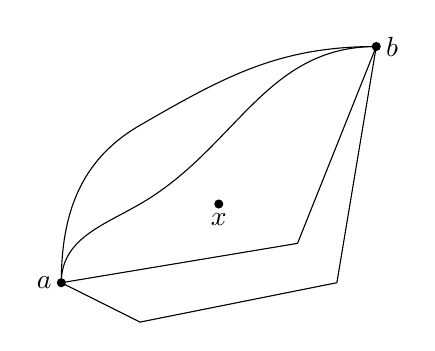
\begin{tikzpicture}
    \draw[fill] (0,0) circle [radius=0.05];
    \draw[fill] (-2,-1) circle [radius=0.05];
    \draw[fill] (2,2) circle [radius=0.05];
    \node [below] at (0,0) {$x$};
    \node [left] at (-2,-1) {$a$};
    \node [right] at (2,2) {$b$}; 
    \draw (-2,-1) -- (1,-0.5) -- (2,2);
    \draw (-2,-1) -- (-1,-1.5) -- (1.5, -1) -- (2,2);
    \draw (-2,-1) to [out=90, in=-150] (-1,0);
    \draw (-1,0) to [out=30, in=180] (2,2);
    \draw (-2,-1) to [out=90, in=-150] (-1,1);
    \draw (-1,1) to [out=30, in=180] (2,2);
    \end{tikzpicture}
\end{figure}

This shows that $\R^2\backslash\{x\}$ is path connected and therefore connected.
\end{proof}

\medskip

(b) Using (a), or otherwise, show that $\R$ is not homeomorphic to $\R^2$.

% Note: A homeomorphism between two metric spaces $X$ and $Y$ is a bijection $f:X\ra Y$
% such that both $f$ and $f^{-1}$ are continuous. 

\begin{proof}
Suppose $\R$ is homeomorphic to $\R^2$, then there is a bijection $f: \R \ra \R^2$
such that both $f$ and $f^{-1}$ are continuous. 

Suppose $y = f(x)$. Consider a connected subset of $\R^2$: $\R^2\backslash\{y\}$. 
As shown in part (a), $\R^2\backslash\{y\}$ is connected. 
Since $f^{-1}$ is continuous, it follows that 
$f^{-1}(\R^2\backslash\{y\}) = (-\infty, x)\cup (x,+\infty)$ is also connected.

But only intervals in $\R$ are connected. So it is a contradiction. 
Therefore, $\R$ is not homeomorphic to $\R^2$.
\end{proof}

\medskip

(c) Using (b), or otherwise, show that the circle $\S^1 = \{z\in\R^2: |z|=1\}$ and the sphere 
$\S^2=\{w\in\R^3:|w|=1\}$ are not homeomorphic. 

%Hint: You can reduce this to (b). 

\begin{proof}
Suppose $f: \S^1 \to \S^2$ is a homeomorphism. Let $a,b \in\S^1$ and $a\neq b$.
Then $ f: \S^1 \setminus \{a,b\} \to \S^2 \setminus \{f(a), f(b)\} $
should preserve connectedness. 
However, $\S^2 \setminus \{f(a), f(b)\}$ is connected but $\S^1 \setminus \{a,b\}$ is not.
Therefore, $\S^1$ and $\S^2$ are not homeomorphic.
\end{proof}
\medskip

% Note: Here is something to think about; it is not part of the assignment. 

% Is $\R^2$ homeomorphic to $\R^3$? More generally, is $\R^m$
% homeomorphic to $\R^n$ for $m\neq n$? One can also ask the same questions for spheres.  
% You can probably guess the answers, but almost certainly you will not be able 
% to prove them!



\end{document}


